\section{Results}
\label{sec:Res}

% ----------------------------------------------------------------------- %
% ----------------------------------------------------------------------- %
\subsection{General estimation results}
\label{sec:feasest}

On FA level, 

















% NOTES:
% - 1) address feasibility of estimations for each estimator
% - 2) give general overview about estimation results (see Breidenbach) before going into more detail
%

% Feasibility: 
% FA-level: for 44 out of 45 FA-units, the full model could be applied. For one remaining, only the model without tree species was applied.
% 
% FR-level: 
%
% mathemat. feasibility:
% - op-estimation feasible for 388 of the 405 fu-units. --> for 17 fus not possible due to n2G < 2
% - psmall / extpsynth possible for 386 of the 405 units (for 19 fus not possible). Reason: for 19 fus we have n2G < 2
% - psynth not possible for 403 of 405. For 2 units not possible due to n1G < 2 (these two are included in the 19 above).
%    -> basically, for these 2 fu-units, none of the estimators could produce estimations due to n1G < 2
%  
%  restriction of unbiased estimtors to n2G >= 4: 
% - psmall / extpsynth: 65 of the 386 fu-units have n2G < 4, so theyx cancel out. Thus we have 19 + 65 = 84 fu-units for which no psmall & extpsynth estimations were deliverable.
%   ==> Thus, we have unbiase estimations for 321 of 405 fu units (79%)

% Some stats:
%
%
%
%
%






\newpage
% ----------------------------------------------------------------------- %
% ----------------------------------------------------------------------- %
\subsection{Estimation errors}
\label{sec:esterr}

On both small area levels, the design-unbiased estimators \psmall{} and \extpsynth{} led to a substantial reduction in the estimation errors compared to the SRS estimator (fig. \ref{fig:disterrors}). On the FA level, the SRS estimator yielded an estimation error of 6.7\% on average compared to 5.2\% and 4.8\% under the \extpsynth{} and \psmall{} estimator. The cumulative error distribution (fig. \ref{fig:disterrors}, left) reveals that under the SRS estimator, errors $\leq$ 5\% were achieved for 17\% of the FA units (8 of 45). This proportion could be increased to 62\% (28 FA units) and 73\% (33 FA units) by application of \psmall{} and \extpsynth{}. 95\% of all estimates exhibited errors $\leq$ 9.5\% under the SRS estimator and $\leq$ 6.6\% when using \psmall{} or \extpsynth{}. Estimation errors higher than 10\% only appeared twice for each of the unbiased estimators.\par

The error reduction by the unbiased double sampling estimators was even more pronounced on the FR level (fig. \ref{fig:disterrors}, right), although the overall error niveau was substantially higher than on FA level. The average error under the SRS estimator was 18.3\%, while it was 11.3\% and 12.2\% under the \psmall{} and \extpsynth{} estimator. 95\% of the 321 FR units where \psmall{} and \extpsynth{} could be applied exhibited errors $\leq$ 20\%. In comparion, the SRS estimates resulted in errors $\leq$ 36.6\% for 95\% of the 388 FR units and exceeded an error of 20\% in 30\% of the cases.\par

On both small area levels, the \psynth{} estimator resulted in much smaller estimation errors compared to \psmall{} and \extpsynth{}. This was as expected, since the \psynth{} variance estimate does not take the residual variation in each small area unit into account (section \ref{sec:psynth}). Compared to the error distribution of the asymptotically design-unbiased estimators \psmall{} and \extpsynth{}, the estimation errors of \psynth{} might thus be to optimistic.

\begin{figure}[H]
	\centering
	\resizebox{1\hsize}{!}{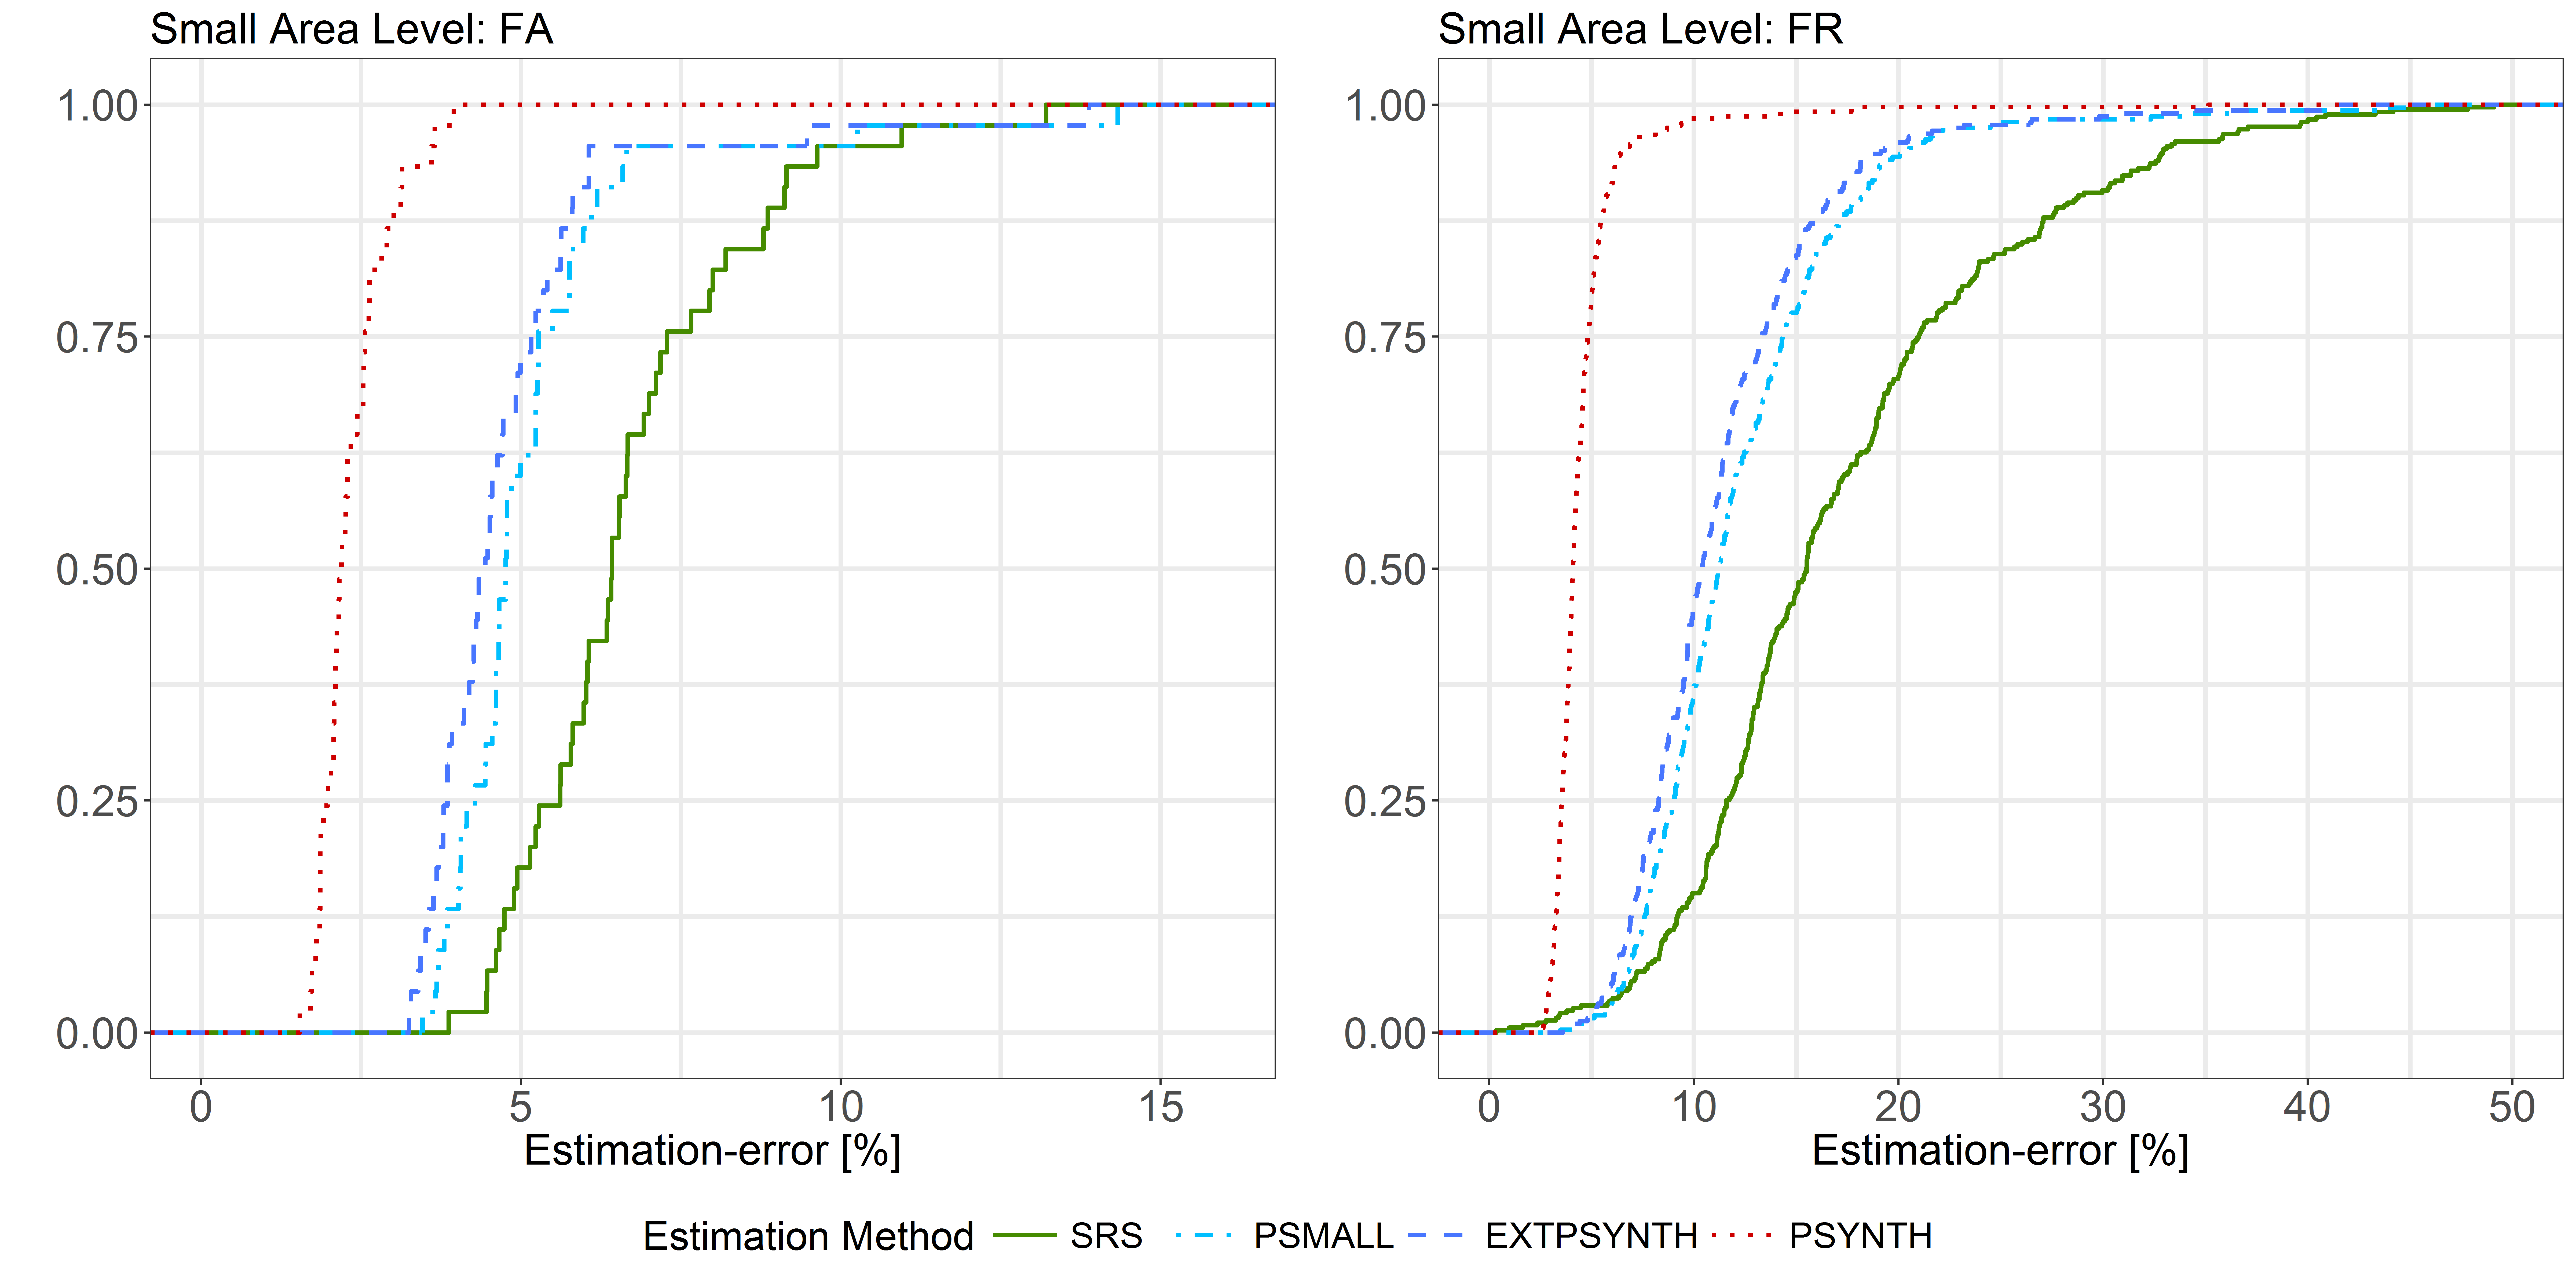
\includegraphics{fig/error_distr_foa_fu.png}}
	\caption{Cumulative distribution of estimation errors under the simple random sampling (SRS), the pseudo small (\psmall{}), the extended pseudo synthetic (\extpsynth{}) and the pseudo synthetic (\psynth{}) estimator. \textit{Left}: Results for the 45 FA units. \textit{Right}: Results for the 388 (SRS), 321 (\psmall{} / \extpsynth{}) and 403 (\psynth{}) FR units.}
	\label{fig:disterrors}
\end{figure}

%% NOTES
 %Estimation errors smaller than 10\% were achieved for only 15\% (xx) of all FR units under SRS, while this proportion could be increased to 38\% and 46\% by PSMALL and EXTPSYNTH. 

% Whereas the estimation errors under PSMALL and PSYNTH were limited to maximum of 41 and 45\%, The SRS estimates exceeded this value in 11 FR units.
%
% AS obvious from figure \ref{fig:disterrors} (right), the major improvement 
%
%
%
%
% The PSYNTH estimator always resulted in much smaller estiamtion errors compared to PSMALL and PSYNTH. This is because ...
%
% As obvious from figure \ref{fig:disterrors}, the error distribution of PSMALL and EXTPSYNTH were found to be very similar and suggested that the two estimator performed very similar. In section \ref{sec:comp}, we analysed the differences between the two estimators in more detail.
%
%The highest observed estimation error was 14\% for the SRS, PSMALL and EXTPSYNTH estimator.



\newpage
% ----------------------------------------------------------------------- %
% ----------------------------------------------------------------------- %
\subsection{Comparison of \psmall{} and \extpsynth{}}
\label{sec:comp}

As obvious from figure \ref{fig:disterrors}, the error distribution of \psmall{} and \extpsynth{} were found to be very similar, with \psmall{} showing marginally higher estimation errors. In order to investigate the differences between \psmall{} and \extpsynth{}, we compared the g-weight variances of both estimators for all 321 FR units (fig. \ref{fig:compvar}, left). As obvious, \psmall{} yielded slightly larger variances for the vast majority of the estimates. As addressed in section \ref{sec:extpsynth}, one possible explanation for such differences was the effect of one or more cluster not entirely being included in a small area unit, as this would constitute a violation of the \extpsynth{} estimator. This violation was actually observed in 155 of the 321 FR units (48\%). However, the affected FR units (depicted in red color, fig. \ref{fig:compvar}) did not show a significant divergence from the \psmall{} variances with respect to the remaining unaffected FR units. The variance differences between the two estimators were expected to occur for the following reason: as depicted in \citet[pp.17--18]{mandallaz2016}, the mathematical formulations of the \psmall{} and \extpsynth{} estimator are asymptotically equivalent only under large terrestrial sample sizes $n_{2,G}$ within the small area. An additional comparison of the absolute differences in the g-weight variance (fig. \ref{fig:compvar}, right) revealed that large differences did in fact particularly occur for small area units with small terrestrial sample sizes ($n_{2,G} \leq 5$). The differences decreased with increasing sample size and thus confirmed the asymptotic relationship between the two estimators. However, a comparison of the confidence intervals of \psmall{} and \extpsynth{} revealed that the variance differences did not lead to statistically significant point estimates.\par

%As obvious from figure \ref{fig:disterrors}, the error distribution of \psmall{} and \extpsynth{} were found to be very similar, with \psmall{} showing marginally higher estimation errors. Differences between the two estimators were expected to occur for the following reasons: 1) as depicted in \citet[pp.17--18]{mandallaz2016}, the mathematical formulations of the \psmall{} and \extpsynth{} estimator are asymptotically equivalent only under large terrestrial sample sizes $n_{2,G}$ within the small area. Therefore, differences between the estimators were particularly expected for small area units with low terrestrial sampling intensities. 2) As addressed in section \ref{sec:extpsynth}, the case of one or more cluster not entirely being included in a small area unit would constitute a violation of the \extpsynth{} estimator. Effects of this violation on the estimates had yet not been investigated and also lead to a divergence between \psmall{} and \extpsynth{}.\par
%
%In order to investigate the differences between \psmall{} and \extpsynth{}, we compared the g-weight variances of both estimators for all 321 FR units (fig. \ref{fig:compvar}, left). As obvious, \psmall{} yielded slightly larger variances for the vast majority of the estimates. A violation of the \extpsynth{} assumption by one or more cluster not entirely included in a small area unit was observed in 155 of the 312 FR units (48\%). However, the affected FR units (depicted in red color, fig. \ref{fig:compvar}) did not show a significant divergence from the \psmall{} variances with respect to the remaining unaffected FR units. An additional comparison of the absolute differences in the g-weight variance (fig. \ref{fig:compvar}, right) revealed that large differences particularly occurred for small area units with small terrestrial sample sizes ($n_{2,G} \leq 5$). The differences decreased with increasing sample size and thus confirmed the asymptotic relationship between the two estimators. A comparison of the confidence intervals of \psmall{} and \extpsynth{} revealed that the variance differences did not lead to statistically significant point estimates.\par



% NOTES:
% - Section \ref{sec:comp} provides a more detailed analysis of the differences between the two estimators.
% - DM-explanation: The model residuals and thus the residual variance for extpsynth should in general be a bit better than those of psmall, since we additionally adjust the regression
%                   to the small area data by introducing the sae-indicator variable (even if this is strictly speaken only a means to cause zero-mean-residuals)
%                   ==> we even can relate the differences to the residual variation, since the first and second term of extpsynth and psmall area identical with exception 
%                       of the adjusted regression coefficient
% - we can see the asymptotic of psmall and extpsynth: with increasing n2G, psmall and extpsynth are mathematically identical
% ==> so differences will particularly concern sae units with small n2G (threshold seems to be around n2G < 10)
%
% for Discussion:
% - our analyses 
%   a) suggest that the differences between \psmall{} and \extpsynth{} become negligible for sample sizes $n_{2,G}$ larger than 10 due to the asymptotic relationship between these estimators 
%   b) showed that violation of the '\extpsynth{}'-assumption had only minor effects on the variance estimates that did not lead to statistically different point estimates 
%   c) indicate that \extpsynth{} will in general have slightly smaller est.variances due to a slightly better model fit through the data in the small area, which is caused by the 
%      adjusted intercept (which however is mainly a means to insure the zero-mean-residual assumption in the \extpsynth{}-estimator


\begin{figure}[H]
	\centering
	\resizebox{1\hsize}{!}{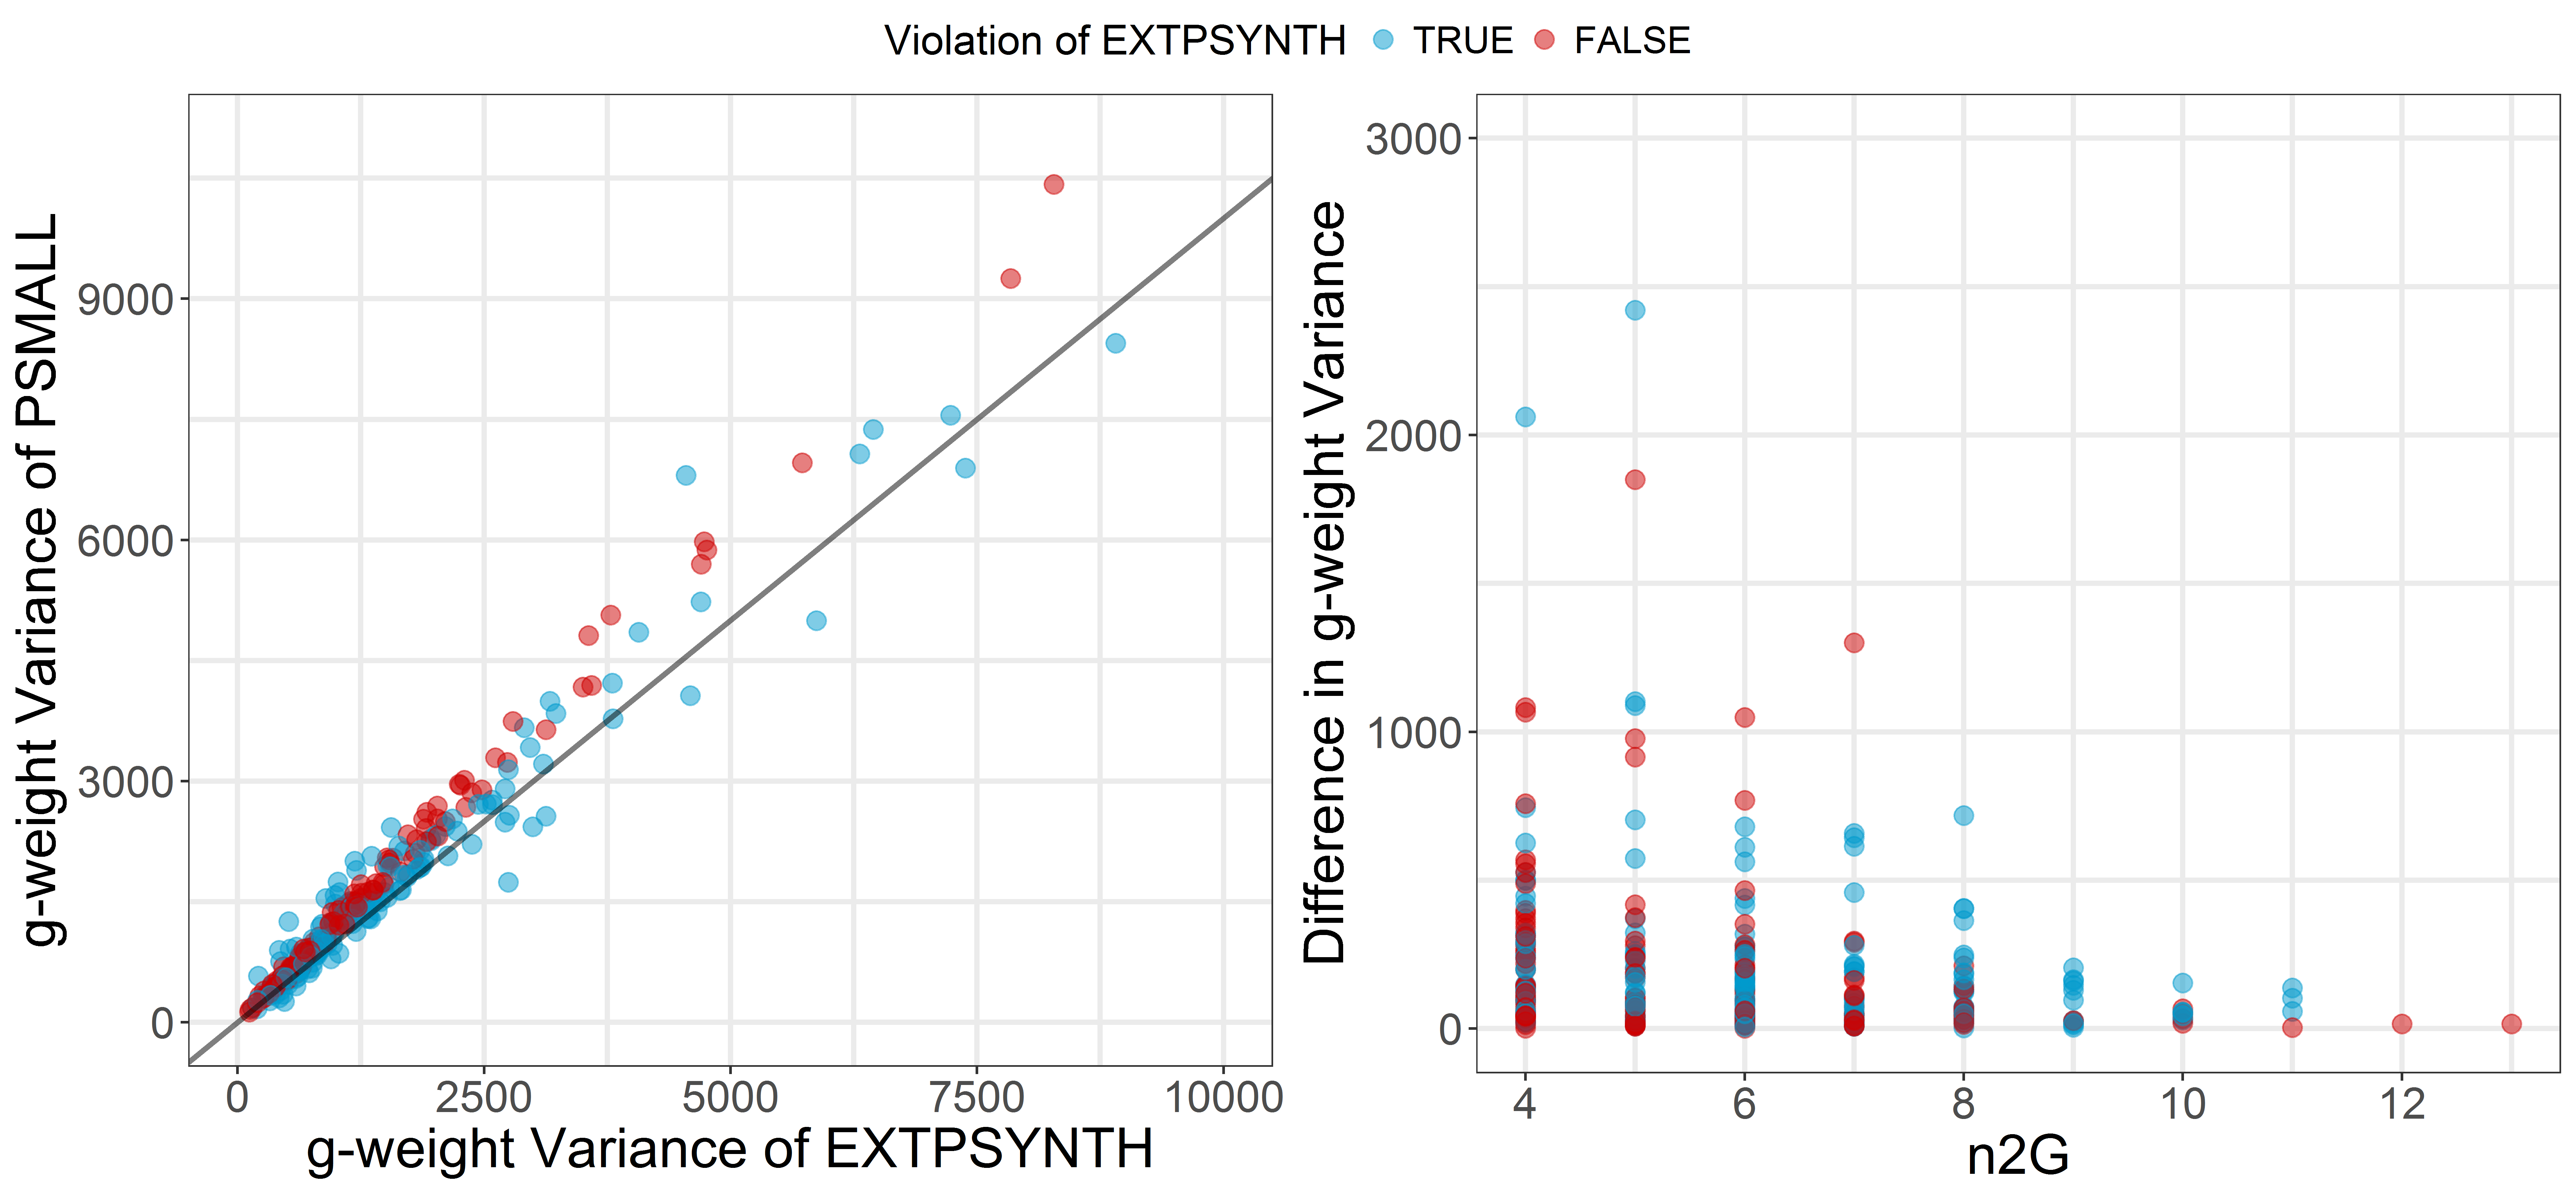
\includegraphics{fig/psmall_vs_extpsynth_fu.png}}
	\caption{\textit{Left}: Comparison of the g-weight variance between the PSMALL and the EXTPSYNTH estimator for the 321 FR units.
		\textit{Right}: Difference in g-weight variance between the PSMALL and the EXTPSYNTH estimator in dependence of the terrestrial data ($n2G$) in the FR unit.}
	\label{fig:compvar}
\end{figure}


\newpage
% ----------------------------------------------------------------------- %
% ----------------------------------------------------------------------- %
\subsection{Reduction of variance by two-phase estimators}
% \subsection{Variance reduction of SRS estimator}
\label{sec:gain_eval}




\begin{figure}[H]
	\centering
	\resizebox{0.7\hsize}{!}{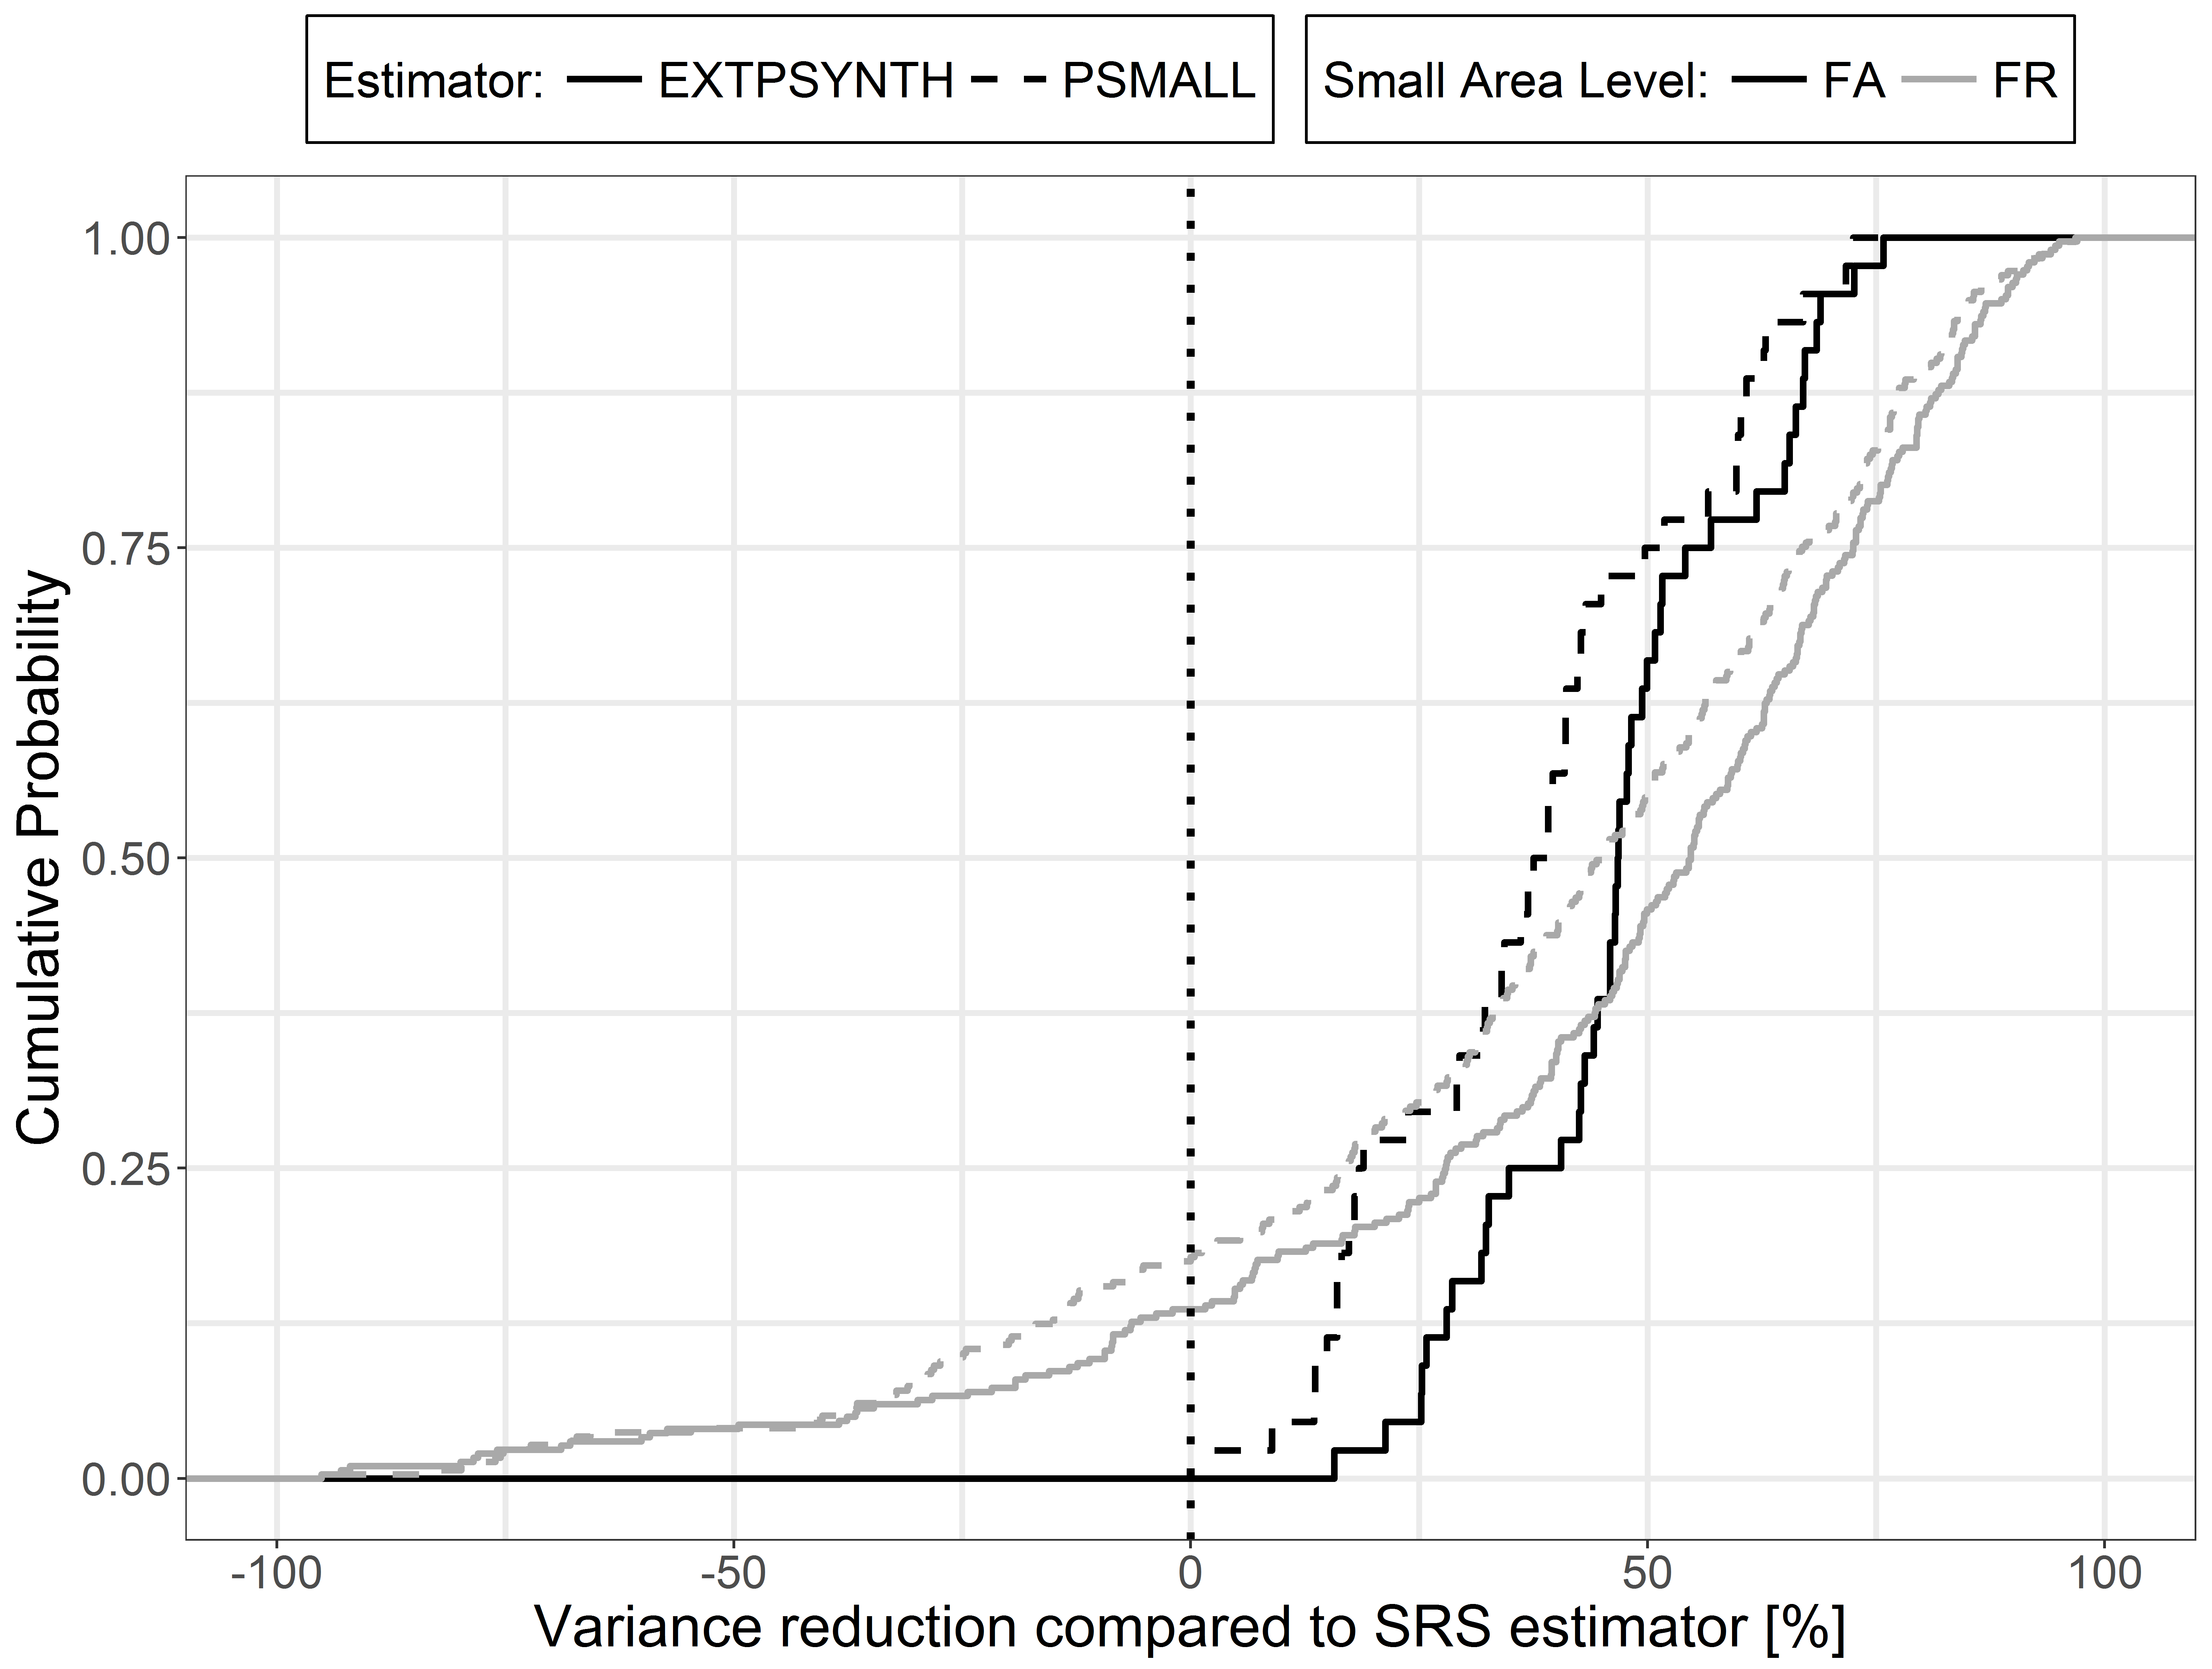
\includegraphics{fig/compare_onephase_extpsynth_psmall.png}}
	\caption{Cumulative distribution of variance reduction by the PSMALL and EXTPSYNTH compared to the SRS estimator for the  45 FA and 321 FR units.}
	\label{fig:gain}
\end{figure}





\begin{figure}[H]
	\centering
	\resizebox{0.7\hsize}{!}{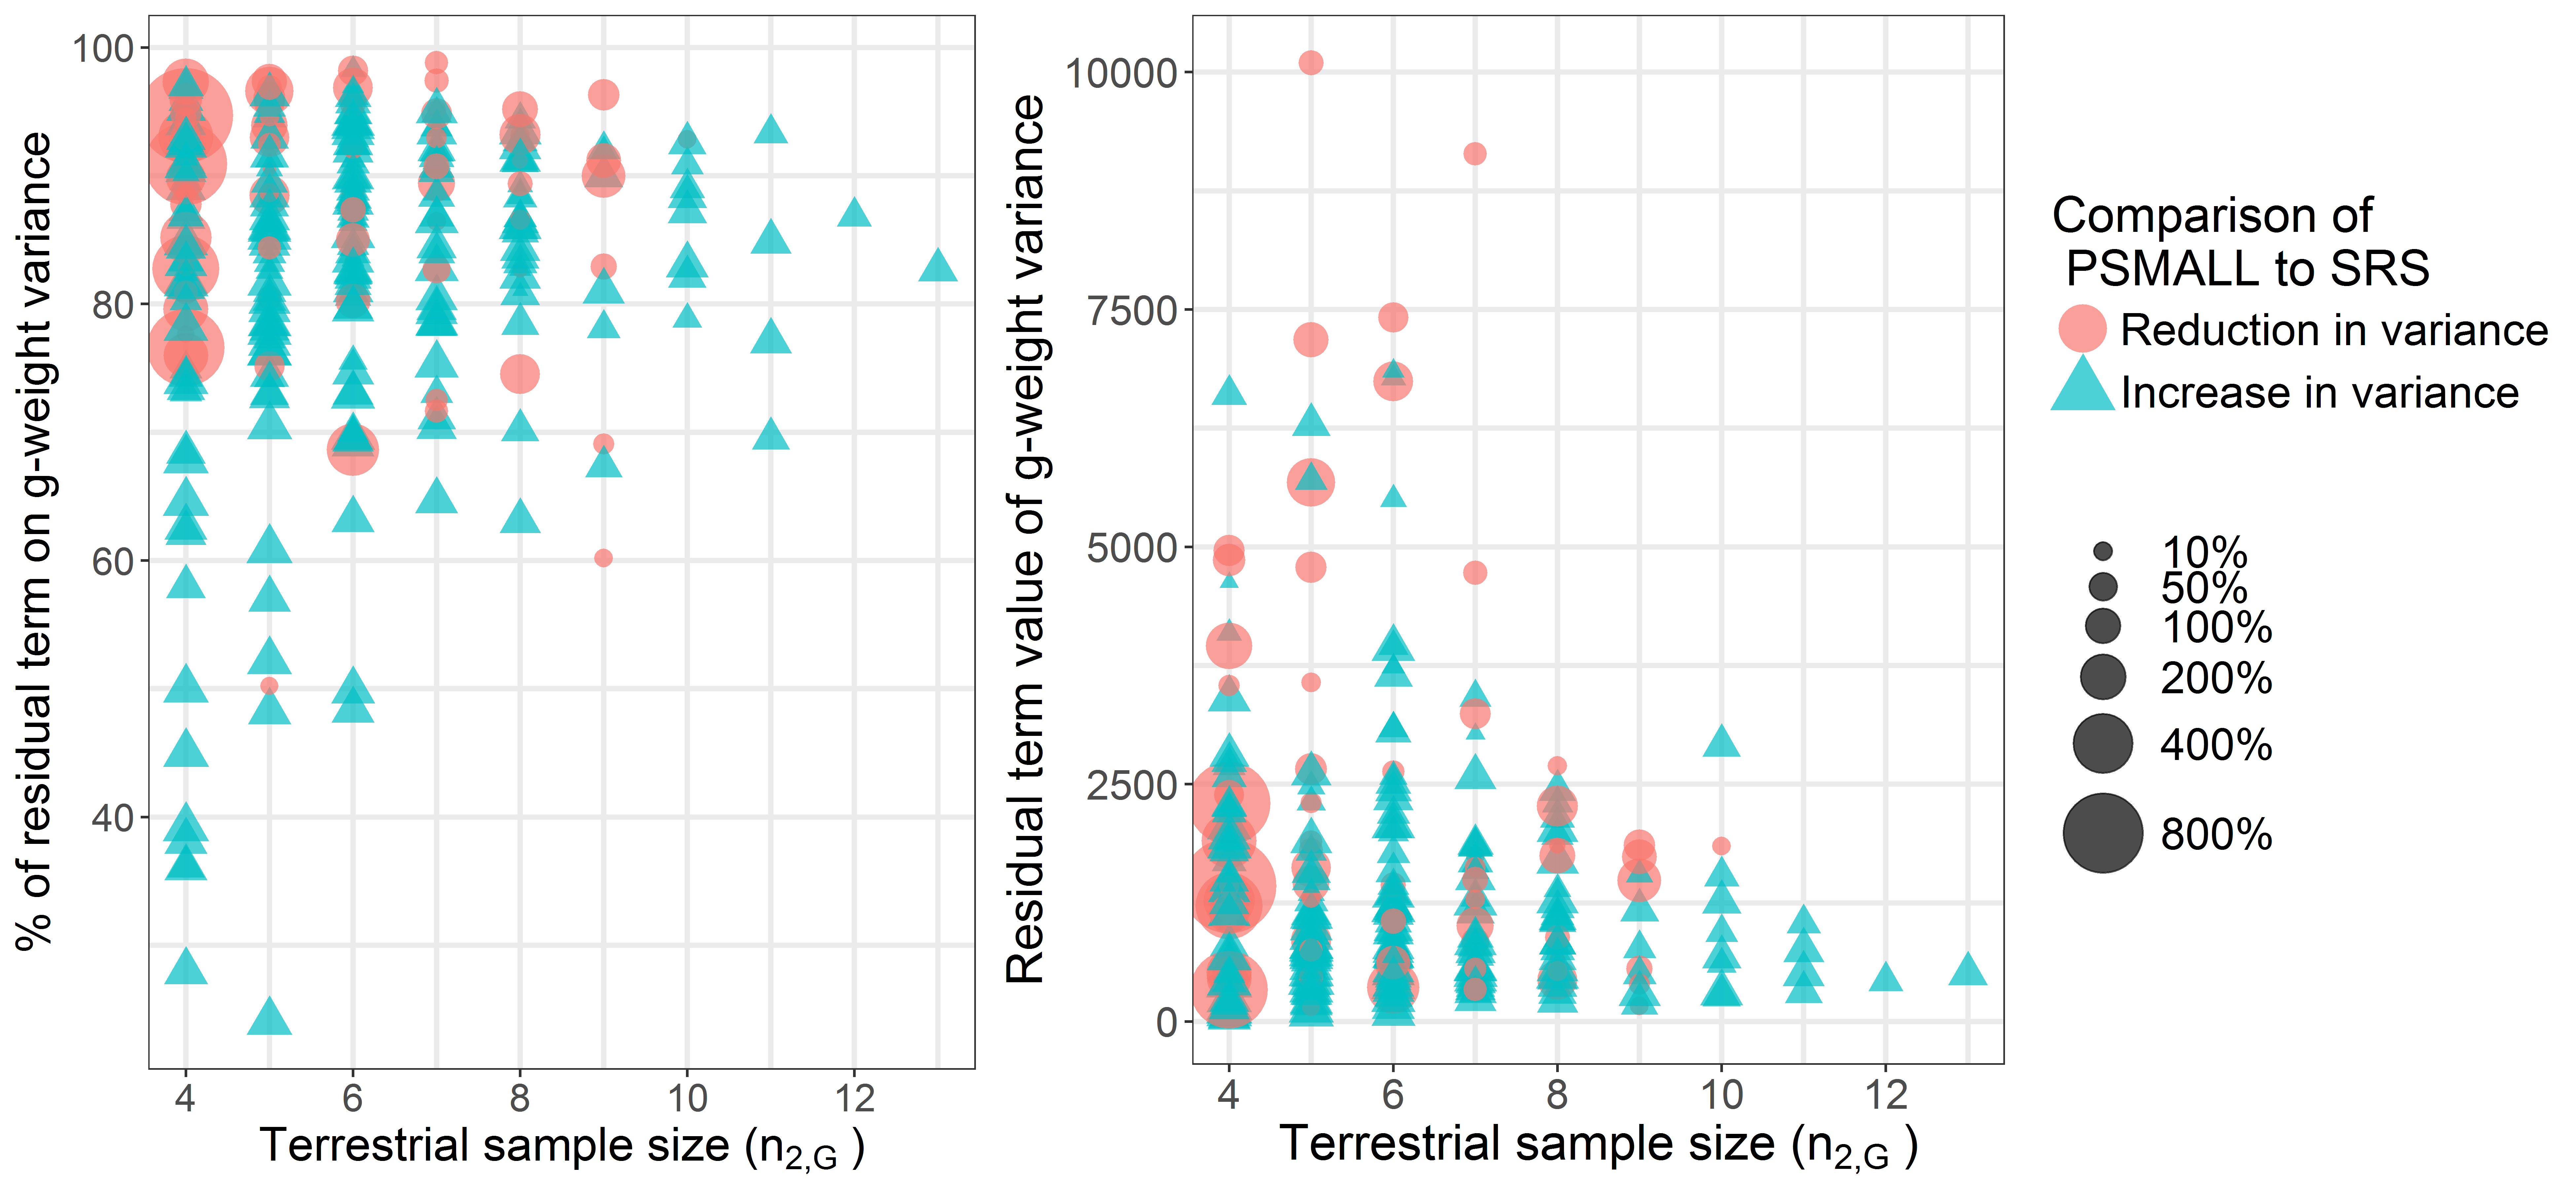
\includegraphics{fig/eval_2phase_fail.png}}
	\caption{}
	\label{fig:fail}
\end{figure}


%% NOTES:
% - 
%
%
%
%
%
%
%








